\documentclass{article}

%%% Packages %%%

\usepackage[margin=1in]{geometry}
\usepackage{exercise}
\renewcommand{\ExerciseHeader}{%
  \par\noindent
  \textbf{\large \ExerciseName{} \, \ExerciseHeaderNB\ExerciseHeaderTitle\ExerciseHeaderOrigin}%
  \par\nopagebreak\medskip
}
\usepackage[utf8]{inputenc}
\usepackage[T1]{fontenc}
\usepackage{amsmath, amsfonts, amssymb, stmaryrd, bbold, url, hyperref}
\usepackage[version=4]{mhchem}
\usepackage{graphicx}

%%% Commands %%%

\newcommand{\proba}[1]{\mathbb{P}[#1]}
\newcommand{\var}[1]{\operatorname{Var}[#1]}
\newcommand{\esperance}[1]{\mathbb{E}[#1]}
\newcommand{\limitinftyn}{\xrightarrow[n \to{} \infty]{}}
\newcommand{\indicator}[1]{\mathbb{1}_{#1}}
\newcommand{\R}{\mathbb{R}}

%%% Solutions %%%

\newtheorem{solution}{Solution}
\newif\ifhidesolutions{}
% \hidesolutionstrue %decommenter pour cacher les SOLUTIONS

\ifhidesolutions{}
\usepackage{environ}
\NewEnviron{hide}{}
\let\solution\hide{}
\let\endsolution\endhide{}
\fi

%%% Title %%%

\title{PC 2 --- Probability distributions}
\author{}
\date{}

%%% Document %%%

\begin{document}

\begin{flushleft}
  \textbf{Probability Refresher} \hfill \textbf{September 2023} \\
  \textbf{Master X-HEC} \hfill \textbf{C. Deslandes, A. Loison,} \\
  É\textbf{cole Polytechnique} \hfill \textbf{D. Métivier \& T. Rebafka}
\end{flushleft}

{\let\newpage\relax\maketitle}
\vspace{-1.3cm}
\hrule

\vspace{0.5cm}

\begin{Exercise} (Uniform distribution). Let $X$ be a random variable with uniform distribution on $[0,1]$. We define $Y=\min (X, 1-X)$ and $Z=\max (X, 1-X)$. Determine the distributions of $Y$ and $Z$. Compute $\mathbb{E}[Y Z]$.
\end{Exercise}

\begin{solution}
  La variable al\'{e}atoire $Y$ prend ses valeurs dans $[1/2,1]$ et pour tout $t\in[1/2,1]$,
  \[
    F_Y(t) = \mathbb{P}(U\leq t,1-U\leq t) = \mathbb{P}(U\leq t,U\geq 1-t)
    = t - (1-t) = 2t-1
  \]
  donc $Y$ suit la loi uniforme sur $[1/2,1]$. On remarque que $X = 1-Y$ et on en
  d\'{e}duit que $X$ suit la loi uniforme sur $[0,1/2]$. Pour calculer
  $\mathbb{E}[XY]$, on remarque que $XY = U(1-U)$ et donc
  \[
    \mathbb{E}[XY]
    = \mathbb{E}[U(1-U)]
    = \int_0^{1}\!(t-t^2)\,dt
      = {{[t^2/2-t^3/3]}_0}^{1}
    = 1/2-1/3=1/6.
  \]
\end{solution}

\begin{Exercise}
  One says that $X \in (0,+\infty)$ follows the $\log$-normal distribution if $\log (X) \sim \mathcal{N}(0,1)$. What is the density of $X$?
\end{Exercise}

\begin{solution}
  The density of $X$ is a log normal distribution:
  \[
    f_{X}(x) = \frac{1}{x\sqrt{2\pi}} \exp{\left( -\frac{{(\log(x))}^2}{2} \right)}
  \]
  Indeed,
  \begin{align*}
    F_{\log(X)}(x) & = \proba{\log(X) \leq x}                                                        \\
                   & = \int_{-\infty}^x \frac{1}{\sqrt{2\pi}} \exp{\left( -\frac{x^2}{2} \right)} dt
  \end{align*}
  Therefore,
  \begin{align*}
    F_{X}(x) & = \proba{X \leq x}                                                                                                                     \\
             & = \proba{\log(X) \leq \log(x)}                                                                                                         \\
             & = \int_{-\infty}^{\log(x)} \frac{1}{\sqrt{2\pi}} \exp{\left( -\frac{x^2}{2} \right)} dt                                                \\
             & = \int_{-\infty}^{x} \frac{1}{\sqrt{2\pi}} \exp{\left( -\frac{{\log(u)}^2}{2} \right)} \frac{du}{u} \text{ with new variable } u = e^x
  \end{align*}
  And Therefore
  \[
    f_X(x) = \frac{d}{dx} \left( \int_{-\infty}^{x} \frac{1}{\sqrt{2\pi}} \exp{\left( -\frac{{\log(u)}^2}{2} \right)} \frac{du}{u} \right) = \frac{1}{x\sqrt{2\pi}} \exp{\left( -\frac{{\log(x)}^2}{2} \right)}
  \]
\end{solution}

\begin{Exercise}
  Consider a random variable $X$ having exponential distribution with parameter 1. Let $a>0$ be a positive real number.
  \begin{enumerate}
    \item Compute the cumulative distribution function of $Y=\min (X, a)$. Plot the
          function.

    \item What can you say about the existence of a density for the distribution of $Y$?

    \item Compute $\mathbb{E}[Y]$. Hint: Use $Y=X \mathbb{1}_{X \leq a}+a
            \mathbb{1}_{X>a}$.
  \end{enumerate}
\end{Exercise}

\begin{solution}
  \begin{enumerate}
    \item We have, $\forall t \in \R^+$:
          \begin{align*}
            \proba{Y \geq t} & = \proba{\min(X, a) \geq t}             \\
                             & = \proba{(X \geq t) \cap (a \geq t)}    \\
                             & = \indicator{a \geq t} \proba{X \geq t}
          \end{align*}
          Therefore,
          \[
            \proba{Y \leq t} = 1 - \indicator{a \geq t} \proba{X \geq t}
          \]
          \begin{figure}[h]
            \centering
            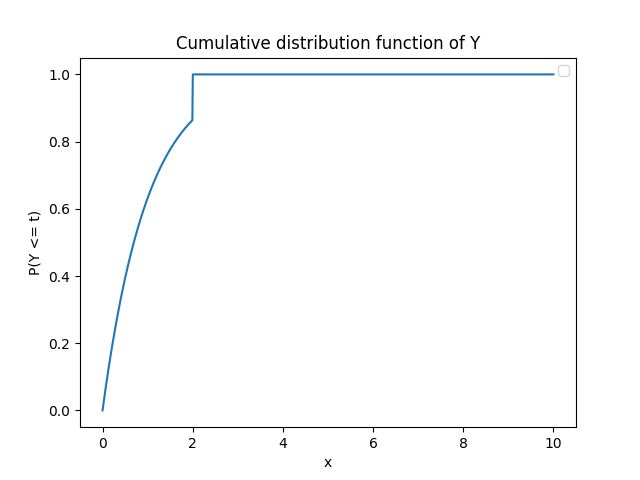
\includegraphics[width=0.6\textwidth]{cdf.png}
          \end{figure}
    \item As the cumulative distribution function is not continuous, the density could not exist: if $X$ has a density $f_X$, $F_X$ should be a continuous function.
    \item We have:
          \begin{align*}
            \esperance{Y} & = \esperance{X \mathbb{1}_{X \leq a} } + a \esperance{\mathbb{1}_{X>a}} \\
                          & = \int_0^a t e^{-t} dt + a \proba{X > a}                                \\
                          & = 1 - (a+1) e^{-a} + a e^{-a}                                           \\
                          & = 1 - e^{-a}
          \end{align*}
  \end{enumerate}
\end{solution}

\begin{Exercise} Let $V$ be a random variable with uniform distribution on $[0, \pi / 2]$. Define the random variable $W=\sin (V)$.
  \begin{enumerate}
    \item Determine the distribution of $W$.
    \item How does the distribution of $W$ change when $V$ has uniform distribution on $[0, \pi]$?
  \end{enumerate}
\end{Exercise}

\begin{solution}
  \begin{enumerate}
    \item We have:
          \begin{align*}
            \proba{W \leq t} & = \proba{\sin(V) \leq t}    \\
                             & = \proba{V \leq \arcsin(t)} \\
                             & = \frac{2 \arcsin(t)}{\pi}
          \end{align*}
    \item Let $0 \leq t \leq 1$ and $\theta \in [0, \frac{\pi}{2}]$ such that
          $\sin(\theta) = t$. If $V$ is uniform on $[0, \pi]$:
          \begin{align*}
            \proba{W \leq t} & = \proba{\sin(V) \leq t}                              \\
                             & = \proba{V \leq \theta} + \proba{V \geq \pi - \theta} \\
                             & = \frac{\theta + \pi - (\pi - \theta)}{\pi}           \\
                             & = \frac{2 \theta}{\pi}
          \end{align*}
          Therefore, the distribution of $\sin(V)$ has not changed.
  \end{enumerate}
\end{solution}

\begin{Exercise} (Cauchy distribution). Let $X$ be a random variable with Cauchy distribution whose density is given by $f(x)={\left(\pi\left(1+x^{2}\right)\right)}^{-1}$. Determine the distribution of $1 / X$ using a change of variables.
\end{Exercise}

\begin{solution}
  Soit $f:\mathbb R\longrightarrow \mathbb R$ continue born\'ee. On a
  \begin{align*}
    \mathbb E[f\left(\frac{1}{X}\right)] & =\int_\mathbb R f\left(\frac1x\right) \frac{1}{\pi(1+x^2)} dx.
  \end{align*}
  On a envie de faire le changement $u=1/x$ (mais pas bijectif sur $\mathbb R$) on scinde en deux

  \begin{align*}
    \mathbb E[f(\frac1X)] & =\int_0^{+\infty} f(\frac1x) \frac{1}{\pi(1+x^2)} dx+ \int_{-\infty}^0 f(\frac1x) \frac{1}{\pi(1+x^2)} dx.
  \end{align*}
  On pose la variable $u=1/x$ donc $du=-u^2 dx$ ainsi
  \begin{align*}
    \int_0^{+\infty} f(\frac1x) \frac{1}{\pi(1+x^2)} dx & =\int_0^{+\infty} f(u)\frac{1}{u^2}  \frac{1}{\pi(1+u^{-2})} du \\
                                                        & =\int_0^{+\infty} f(u) \frac{1}{\pi(1+u^2)} du.
  \end{align*}
  De plus en faisant $u=1/x$ dans l'integrale sur $\mathbb R^-$ on a de m\^eme

  \begin{align*}
    \int_{-\infty}^0 f(\frac1x) \frac{1}{\pi(1+x^2)} dx & =\int_{-\infty}^0 f(u) \frac{1}{\pi(1+u^2)} du.
  \end{align*}
  Donc $\frac1X$ a m\^eme loi que $X$.
\end{solution}

\begin{Exercise}
  Let $p>0$ and an integer $n$ such that $n>p$. Consider random variables $Y_{n}$ such that $n Y_{n}$ has a geometric distribution $\operatorname{Geo}\left(\frac{p}{n}\right)$ with parameter $\frac{p}{n}$. Show that the characteristic function of $Y_{n}$ tends to the characteristic function of an exponentially distributed random variable with parameter $p$.
\end{Exercise}

\begin{solution}
  Let $p_n = \frac{p}{n}$. We have:
  \begin{align*}
    \phi_{Y_n}(t) & = \esperance{e^{itY_n}}                                     \\
                  & = \esperance{e^{i \frac{t}{n} nY_n}}                        \\
                  & = \sum_{k = 1}^\infty p_n e^{i\frac{t}{n}k} {(1-p_n)}^{k-1} \\
                  & = \frac{p_n}{1 - (1-p_n) e^{i\frac{t}{n}}}
  \end{align*}
  But:
  \begin{align*}
    (1-p_n) e^{i\frac{t}{n}} & \sim (1-p_n) (1 + i \frac{t}{n})              \\
                             & = 1 - p_n + i \frac{t}{n} - p_n i \frac{t}{n}
  \end{align*}
  Therefore:
  \[
    1 - (1-p_n) e^{i\frac{t}{n}} = p_n - i \frac{t}{n} + p_n i \frac{t}{n}
  \]
  And finally
  \[
    \frac{p_n}{1 - (1-p_n) e^{i\frac{t}{n}}} \to \frac{p}{p - it}
  \]
  And if $X \sim Exp(p)$:
  \begin{align*}
    \phi_{X}(t) & = \esperance{e^{itX}}                                 \\
                & = \sum_{k = 0}^\infty p e^{itk} e^{-p} \frac{p^k}{k!} \\
                & = \frac{p}{p-it}
  \end{align*}
  which conclude the execise.
\end{solution}

\begin{Exercise} Let $\alpha>1$ be fixed. Consider the random variable $X$ with density given by
  \[
    f(x)=c_{\alpha} x^{-\alpha} \mathbb{1}_{x \geq 1}
  \]
  \begin{enumerate}
    \item Determine the constant $c_{\alpha}$.
    \item For which values of $p$ we have $X$ belongs to $L^{p}$?
  \end{enumerate}
\end{Exercise}

\begin{solution}
  \begin{enumerate}
    \item Necessarily, $\int_\R f(x) = 1$. So:
          \begin{align*}
                 & \int_\R c_{\alpha} x^{-\alpha} \mathbb{1}_{x \geq 1} dx = 1
            \iff & c_{\alpha} \int_1^\infty x^{-\alpha} dx = 1
            \iff & c_{\alpha} = \frac{-1}{\frac{1}{1-\alpha}}                  \\
            \iff & c_{\alpha} = \alpha - 1
          \end{align*}
    \item We have:
          \begin{align*}
            X \in L^p & \iff \esperance{X^p} < \infty                                  \\
                      & \iff \int_\R x^p x^{-\alpha} \mathbb{1}_{x \geq 1} dx < \infty
                      & \iff \int_1^\infty x^{p-\alpha} dx < \infty                    \\
                      & \iff p - \alpha < -1
          \end{align*}
          To understant the last step, see \url{https://boilley.ovh/cours/integrale-generalisee.html}.
          And finally the nessary and sufficient condition is $p - \alpha < -1$.
  \end{enumerate}
\end{solution}

\begin{Exercise} Let $X$ and $Y$ be two independent random variables such that $X$ (resp. $Y$) has geometric distribution with parameter $p$ (resp. $q$).
  \begin{enumerate}
    \item Compute $\mathbb{P}(X>n)$ for any $n \in \mathbb{N}$.
    \item What is the distribution of the random variable $Z=\min (X, Y)$?
  \end{enumerate}
\end{Exercise}

\begin{solution}
  \begin{enumerate}
    \item We have:
          \begin{align*}
            \proba{X > n} & = \sum_{k = n+1}^\infty p {(1-p)}^{k-1} \\
                          & = {(1-p)}^n
          \end{align*}
          using a formula for the sum of geometric terms.
    \item Let determine the value of $\proba{\min(X, Y) = k}$.
          \begin{align*}
            \proba{\min(X, Y) = k} & = \proba{(X = k \cap Y > k) \cup (X > k \cap Y = k) \cup (X = k \cap Y = k)}      \\
                                   & = \proba{X = k \cap Y > k} + \proba{X > k \cap Y = k} + \proba{X = k \cap Y = k}  \\
                                   & = p {(1-p)}^k {(1-q)}^{k} + {(1-p)}^{k} q {(1-q)}^{k} + p {(1-p)}^k q {(1-q)}^{k} \\
                                   & = {(1-p)}^k {(1-q)}^k (p + q + pq)
          \end{align*}
  \end{enumerate}
\end{solution}

\begin{Exercise} Assume that $X \sim \mathcal{N}\left(\mu, \sigma^{2}\right)$.
  \begin{enumerate}
    \item Show that $Y=(X-\mu) / \sigma$ has standard normal distribution
          $\mathcal{N}(0,1)$.
    \item Compute $\mathbb{E}[|Y|]$ and $\mathbb{E}\left[Y^{2019}\right]$.
  \end{enumerate}
\end{Exercise}

\begin{solution}
  \begin{enumerate}
    \item If $Y=(X-\mu)/\sigma$, then:
          \begin{align*}
            \proba{a \leq Y \leq b} & = \proba{a \leq \frac{X-\mu}{\sigma} \leq b}                                                                     \\
                                    & = \proba{a\sigma + \mu \leq X \leq b\sigma + \mu}                                                                \\
                                    & = \int_{a\sigma + \mu}^{b\sigma + \mu} \frac{1}{\sqrt{2\pi \sigma^2}} e^{-\frac{{(x-\mu)}^2}{2\sigma^2}} dx      \\
                                    & = \int_a^b \frac{1}{\sqrt{2\pi}} e^{-\frac{y^2}{2}} dy \text{ with change of variable } y = \frac{x-\mu}{\sigma}
          \end{align*}
          Therefore, $Y$ follows a normal distribution.
    \item Let compute $\esperance{|Y|}$.
          \begin{align*}
            \esperance{|Y|} & = \frac{1}{\sqrt{2\pi}} \int_\R |x| e^{\frac{-x^2}{2}}                \\
                            & = \frac{1}{\sqrt{2\pi}}.2. \int_{\R^+} x e^{\frac{-x^2}{2}}           \\
                            & = \sqrt{\frac{2}{\pi}} {{\left[ e^{\frac{-x^2}{2}} \right]}_0}^\infty \\
                            & = \sqrt{\frac{2}{\pi}}
          \end{align*}
          As the distribution of $Y$ is even, the expected value of $Y^{2019}$ should be zero:
          \begin{align*}
            \esperance{Y^{2019}} & = \frac{1}{\sqrt{2\pi}} \int_\R x^{2019} e^{\frac{-x^2}{2}} \\
                                 & = 0
          \end{align*}
  \end{enumerate}
\end{solution}

\end{document}